\documentclass{achemso}
\usepackage[utf8]{inputenc}
\usepackage[dvipsnames]{xcolor}
\usepackage{amsmath}
\usepackage{multirow}

\definecolor{richelectricblue}{rgb}{0.03, 0.57, 0.82}
\newcommand{\vv}[1]{{\textbf{\textcolor{red}{Venkat: #1}}}}
\newcommand{\ab}[1]{{\textbf{\textcolor{ForestGreen}{Alec: #1}}}}
\newcommand{\abattention}[1]{{\textbf{\textcolor{Orange}{Alec: #1}}}}
\newcommand{\lf}[1]{{\textbf{\textcolor{richelectricblue}{Leif: #1}}}}
\newcommand{\ssri}[1]{{\textbf{\textcolor{cyan}{SS: #1}}}}
\graphicspath{ {./Figures/} }

\title{Performance Metrics Required of Next-Generation Batteries to Electrify Commercial Aircraft}
\author{Alexander Bills}
\affiliation{%
 Department of Mechanical Engineering, Carnegie Mellon University, Pittsburgh, Pennsylvania 15213\\
}

\author{William Leif Fredericks}
\affiliation{%
 Department of Mechanical Engineering, Carnegie Mellon University, Pittsburgh, Pennsylvania 15213\\
}

\author{Shashank Sripad}
\affiliation{%
 Department of Mechanical Engineering, Carnegie Mellon University, Pittsburgh, Pennsylvania 15213\\
}

\author{Madalsa Singh}
\affiliation{%
 Department of Mechanical Engineering, Carnegie Mellon University, Pittsburgh, Pennsylvania 15213\\
}

\author{Venkatasubramanian Viswanathan*}
\affiliation{%
 Department of Mechanical Engineering, Carnegie Mellon University, Pittsburgh, Pennsylvania 15213\\
}
\email{venkvis@cmu.edu}
\begin{document}


%%%%%INTRODUCTION%%%%%%%%

%\section{Introduction}

Electric aircraft have generated an enormous amount of interest following the success of the electrification of passenger vehicles. Over 4 million passenger electric vehicles have been sold\cite{4millionblog}, and there have been numerous announcements regarding the electrification of SUVs, pick-up trucks and other light commercial vehicles, which represent the majority of the passenger automotive market today. \ab{https://products.rivian.com/} \ssri{take a few links from our conversation piece} However, while electrification of ground vehicles is well underway, electrification of aircraft is still in its infancy. Announcements have been made regarding electric vertical takeoff and landing (eVTOL) aircraft by companies including Uber \cite{elevate}, Airbus \cite{vahana}, and others\cite{cora}. In a recent viewpoint, we identified the challenging battery requirements faced by eVTOL aircraft, reiterating  the obvious importance of specific energy (defined as the energy available per unit mass) and identifying the importance of power limitations and thermal management requirements during take-off and landing. \cite{fredericks2018performance} While eVTOL aircraft represent a new market for electrification, electrifying existing commercial aircraft could reduce the environmental impact of the transportation segment as a whole. Currently, commercial aircraft represent 9\% of the carbon emissions from transportation, and a much higher contribution to the total warming effect as a result of Aircraft-Induced cloud contrails\cite{davis2017transportation}, \cite{AIC}. Efforts are underway towards the development of electric and hybrid-electric commercial aircraft \cite{zunum} \cite{wright},\cite{utc}\vv{cite Zunum, Wright, Pratt, etc}. In addition, countries (e.g. Norway)\cite{norway} are intending to partially or fully electrify their fleet over the next few decades.   Further, the world's largest seaplane operator, Harbor Air, announced their intention to electrify their fleet.\cite{seaplane} However, despite all the announcements and initiatives, numerous technological challenges remain and one of the primary challenges is the performance metrics required of batteries to electrify commercial aircraft.  Several analyses have presented a comprehensive system-level perspective on the challenges and have identified sub-system component targets\cite{Epstein}, \cite{GNADT20191} .  In this viewpoint, we primarily focus on developing a detailed understanding of the performance metrics required of batteries to electrify the commercial aviation market along with a discussion of possible approaches towards meeting these metrics.

One major challenge in identifying battery pack requirements stems from the wide variety of commercial aircraft on the market and thus the associated uncertainty due to this heterogeneity. In our analysis, we divide commercial aircraft into three categories: (i) Regional, (ii) Narrow body, and (iii) Wide body aircraft. Regional aircraft typically fly short missions, about 500 Nautical Miles (nmi) and carry low passenger loads (30-75), while wide body aircraft carry high passenger loads (200-400) and fly much longer missions ($>2000 $ nmi). Narrow body aircraft fall somewhere in between, carrying medium passenger loads and flying ranges of $\sim$1000 nmi. 

%\vv{Trim and move this above.} Previous work on the electrification of commercial aircraft has been focused on conducting performance assessments where hybrid and fully electric aircraft designs have been evaluated for the required battery specific energy and (motors, power systems whatever else). \cite{rosero2007moving, bradley2015subsonic}(add more) \ab{Write some summaries of barrett et. al, etc.}. Rather than calculating the battery requirements of a specific design, we will estimate the battery requirements of each aviation segment. 

%----Intro up to here------%

%----Methods --- 
%\section{Methods}

In the course of a mission, an aircraft takes off, climbs to its cruising altitude, cruises to its destination, descends to near ground level, and then lands\cite{Roskam}. \ab{fixed, leaving comment to easily find} \vv{Why do we do this?  Can it not be integrated -- it should be easy.  Remove this line once we do it.} Commercial aircraft are mandated to maintain emergency reserve energy for contingencies such as diversions or aborted landings. The FAA (Federal Aviation Administration) requires that a commercial aircraft be able to abort a landing, climb to normal cruising altitude, fly to the most distant alternate airport (here assumed to be 200 NMi), and loiter for 45 minutes at normal cruise fuel consumption.\cite{FAAreserve} As an alternative to the extant FAA commercial reserve, a proposed approach is to house the emergency reserve by maintaining an additional 30\% battery state of charge (SoC) \cite{GNADT20191}.We use the 30\% SOC reserve.

To estimate the energy requirement, we use a flight dynamics model which takes an integrated "First Principles" energy and power estimation approach, similar to the one we used to analyze the electrification of light commercial vehicles, \cite{sripad2017evaluation}, semi-trucks, \cite{guttenberg2017evaluating,sripad2017performance}, and eVTOLs \cite{fredericks2018performance}. Four forces act on an aircraft in flight: thrust (force generated by the propulsion system), drag (aerodynamic force opposite to the direction of motion), weight (gravitational force), and lift (aerodynamic force normal to the wings). Power is a function of the geometry and operating conditions of the aircraft, including instantaneous velocity relative to the surrounding airmass (V), zero lift drag coefficient ($C_{D0}$), propulsive efficiency($\eta_{prop}$), mechanical efficiency($\eta_{mech}$), wingloading (S), aspect ratio, and climb or descent angle ($\gamma$).  We assume that at any point in flight, thrust equals drag and lift equals weight. To calculate power at any point during flight,  thrust is multiplied by the velocity, resulting in Equation \ref{eqn:masterPower}\cite{Raymer}. To calculate energy required by the aircraft, the instantaneous power, given in Equation \ref{eqn:masterPower}, is integrated over the duration of the mission. 

\begin{equation}\label{eqn:masterPower}
    \centering
    \mathrm{P = \frac{\frac{1}{2}\ V^3\ S\ C_{D0}\ \rho + \frac{2\ K\ W^2}{\rho\ V\ S} + W\ V\ sin(\gamma)}{\eta_{prop}\ \eta_{mech} }}
\end{equation}
\vv{Explain all the terms in this equation, first.}
\ab{rewrote above paragraph}

Assessing the performance of potential electric aircraft is complicated by the considerable uncertainty of the parameters in Eq. \eqref{eqn:masterPower}. Velocity (V) and induced drag correction factor (K) are dependent on various other parameters detailed in the \textit{Supplementary information}. The remaining parameters, namely, the zero-lift drag coefficient ($C_{D0}$), propulsive efficiency($\eta_{prop}$), mechanical efficiency($\eta_{mech}$), wing loading (S), and aspect ratio\ab{We never really show what aspect ratio is, is this a problem?} can be estimated using existing aircraft specifications for each size. Approaches to handling the uncertainty in the parameters will be discussed later. Further, uncertainty in the mass of aircraft components is also a concern. Rather than estimating individual aircraft component weights as done in earlier work,\cite{GNADT20191} we adopt a simpler approach diving the total weight into a factor, known as the empty weight fraction, which represents the weight of the aircraft mass without batteries and payload to the total mass Eq. \eqref{Eqn:massSum}.

\begin{equation}
    M_{TO} = ewf * M_{TO} + S_e * \int P(t) dt  + M_{pax} 
    \label{Eqn:massSum}
\end{equation}

 Table 1 contains the upper limit, lower limit, and nominal values of the parameters for each category of aircraft. 

\vv{How can we make this parameters more visual?  Could we draw something like a control chart instead?  Much more visual and easy to understand.  We can have the table in the SI.}
\begin{figure}[htp]
\centering

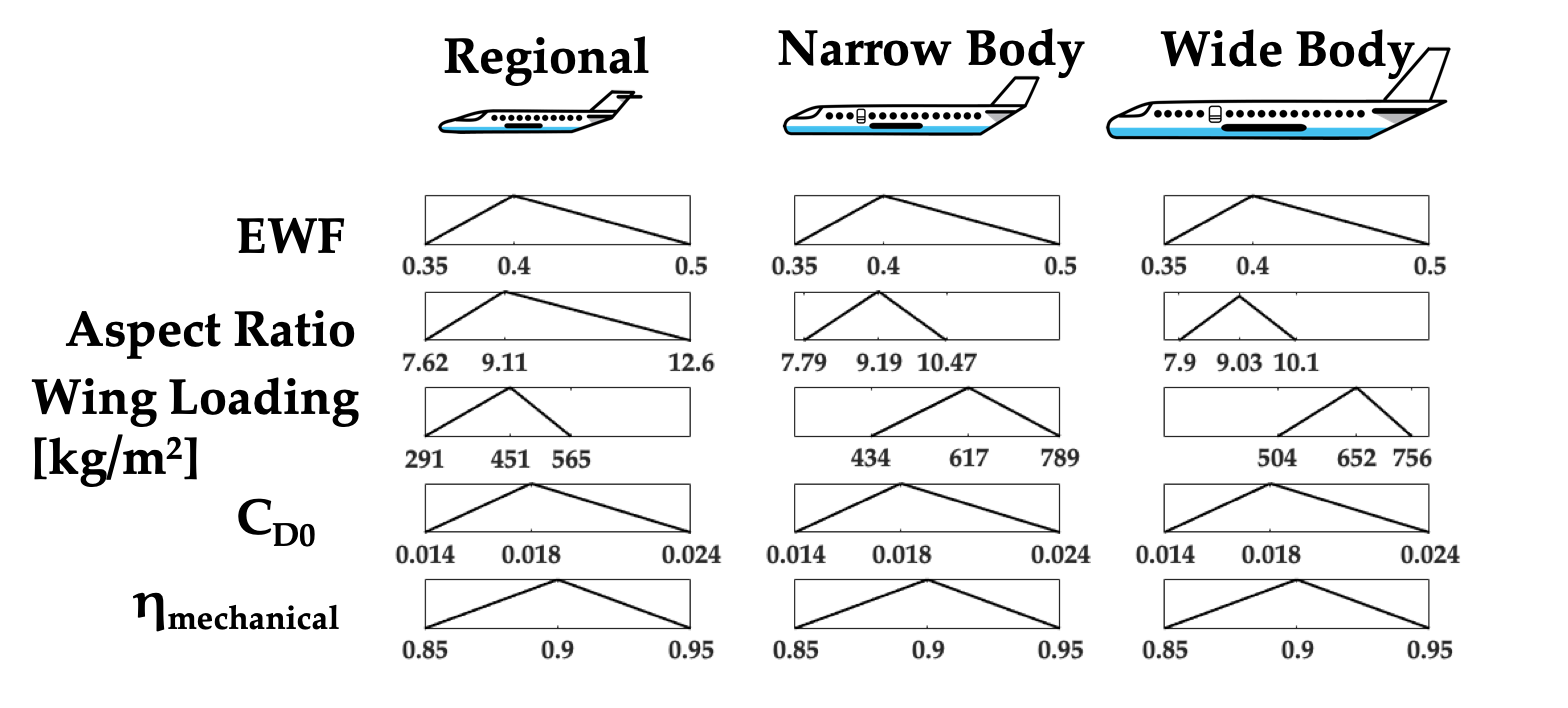
\includegraphics[width=0.8\textwidth]{Figures/chart_figure.png}

\caption{Parameters used to estimate specific energy for various classes of commercial aircraft \textbf{bigcite}}
\label{fig:params}

\end{figure}
%--------Analysis-------------%
%\section{Analysis}


%\subsection{Analysis Method 1: Parameter Uncertainty}
To address uncertainty in the parameters for Equation \eqref{eqn:masterPower}, we perform a monte carlo simulation by sampling each of the parameters in Figure \ref{fig:params}. (\textbf{Change to a reference once we have a final table or a figure}) from a triangular distribution with minimum, mode, and maximum as shown in Figure \ref{fig:params}.\vv{What is the basis for using an uniform distribution?  Triangular maybe better?} The mission for this analysis (i.e. range and payload) was defined a priori, in a Bayesian sense.  The range for a regional aircraft was defined as 350 nmi, for narrow body aircraft, it was 500 nmi, and for wide body aircraft, it was 1000 nmi.  The passenger count for regional aircraft was 75, for narrow body aircraft was 150, and for wide body aircraft was 300. The take off mass for regional aircraft was 50000 Kg, for narrow body aircraft was 100000 Kg, and for wide body aircraft was 250000 Kg.\vv{Add extensive refs for each number.} Figure \ref{fig:histograms} shows the resulting histogram of minimum specific energy, required for a feasible aircraft.

\begin{figure}[htp]
\centering

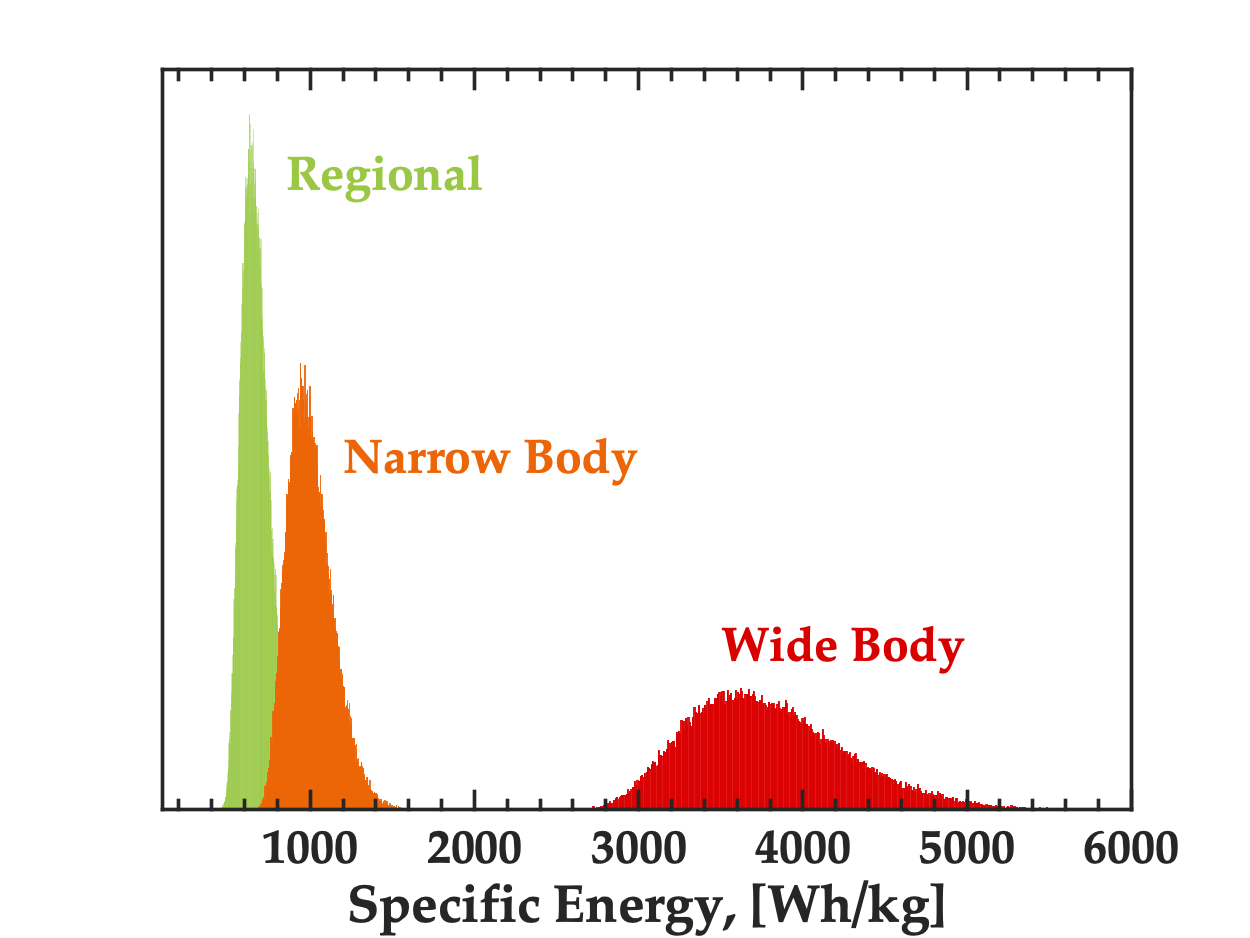
\includegraphics[width=0.6\textwidth]{Figures/histograms.png}

\caption{Histograms of specific energy for regional, narrow body, and wide body aircraft. This figure clearly illustrates the uncertainty resulting from the parameter uncertainty in each aircraft class. The wide body case in particular is extremely uncertain.}
\label{fig:histograms}

\end{figure}

The distribution of required specific energy for regional aircraft has lower and upper bounds of around 475 Wh/kg and 725 Wh/kg. The mode of the distribution is located around 550 Wh/kg. For narrow body aircraft, the lower and upper bounds are around 650 Wh/kg and 975 Wh/kg, respectively while the mode lies around 750 Wh/kg. For the wide body aircraft, the required specific energies are much higher with a lower bound of 2,000 Wh/kg and an upper bound of around 3,500 Wh/kg. The mode for the wide body aircraft is located around 2,500 Wh/kg. These results quantify the wide disparity between the performance metrics required of batteries to electrify regional aircraft and that of larger and longer range aircraft. The mean for the regional case is 670 Wh/kg, while the standard deviation is 85. For the narrow body case, the mean is 1002, and the standard deviation is 133. For the wide body case, the mean is 3784, and the standard deviation is 474. For all cases, the data are skewed right.  
\ab{skewness: RJ: 0.6029 NB: .5814 WB: .5560)}
\ab{kurtosis: RJ: 3.3316 NB: 3.2368 WB: 3.1882)}
\vv{Can we do some analysis on the statistics of the distribution.  Can we run J-B test -- if close to normal, then we should provide mean and std. deviation?  Add a line about how these numbers jive with previous estimates.}    

\vv{Can we write a short paragraph or a table of where a subset of current planes would fall in the specific energy requirement from this analysis.}

It should be noted that satisfying these predefined mission requirements does not guarantee that an aircraft is commercially feasible. Small aircraft, such as regional and some narrow body aircraft, often have cruising ranges that are much lower than their maximum range. However, large aircraft often use a much larger fraction of their maximum range in a typical flight. For example, the \textit{Airbus A319}, a small narrow body aircraft, is most likely to fly a range of around 300 Km (\textbf{change to nmi?}) in cruise, and the distribution of its flights are skewed towards the lower end of its range. On the other hand, a wide body aircraft, such as the \textit{Boeing 777} nearly always flies towards the high end of its range, with a mode cruise length of 4843 Km.(\textbf{change to nmi?}) \cite{SUN2019118}

%\subsection{Analysis Method 2: Contours and Max Pnmi}

Having identified the initial feasibility requirements, we analyze the commercial feasibility of a prospective electric aircraft by studying the mission capabilities as a function of specific energy.  This analysis can be viewed as an approach to analyze as the specific energy of batteries improve, what would be the most promising markets for electric aviation.   All parameters in Eq. \eqref{eqn:masterPower} are set to their nominal values. The product of the number of passengers and the aircraft range (Pnmi) is considered as a figure of merit to study system feasibility at each specified EWF and SE. To ensure that the optimization algorithm does not converge to a corner case (e.g. no passengers and extreme long range or high passengers and extreme short range), we subtract a minimum range and passengers. The minima are different for each class and are set by studying historical aircraft of each class.\vv{Explain more.} We then plot the passengers from the aircraft with the highest Pnmi at each design point on figure \ref{fig:contours}. and the range from that design point on figure \ref{fig:contours}. Regional aircraft are first able to satisfy the minimum requirements for this analysis at a specific energy of around XXX, while narrow body and wide body aircraft are able to satisfy the minimum requirements at a specific energy of around YYY and ZZZ respectively.

\begin{figure}[h]
\centering
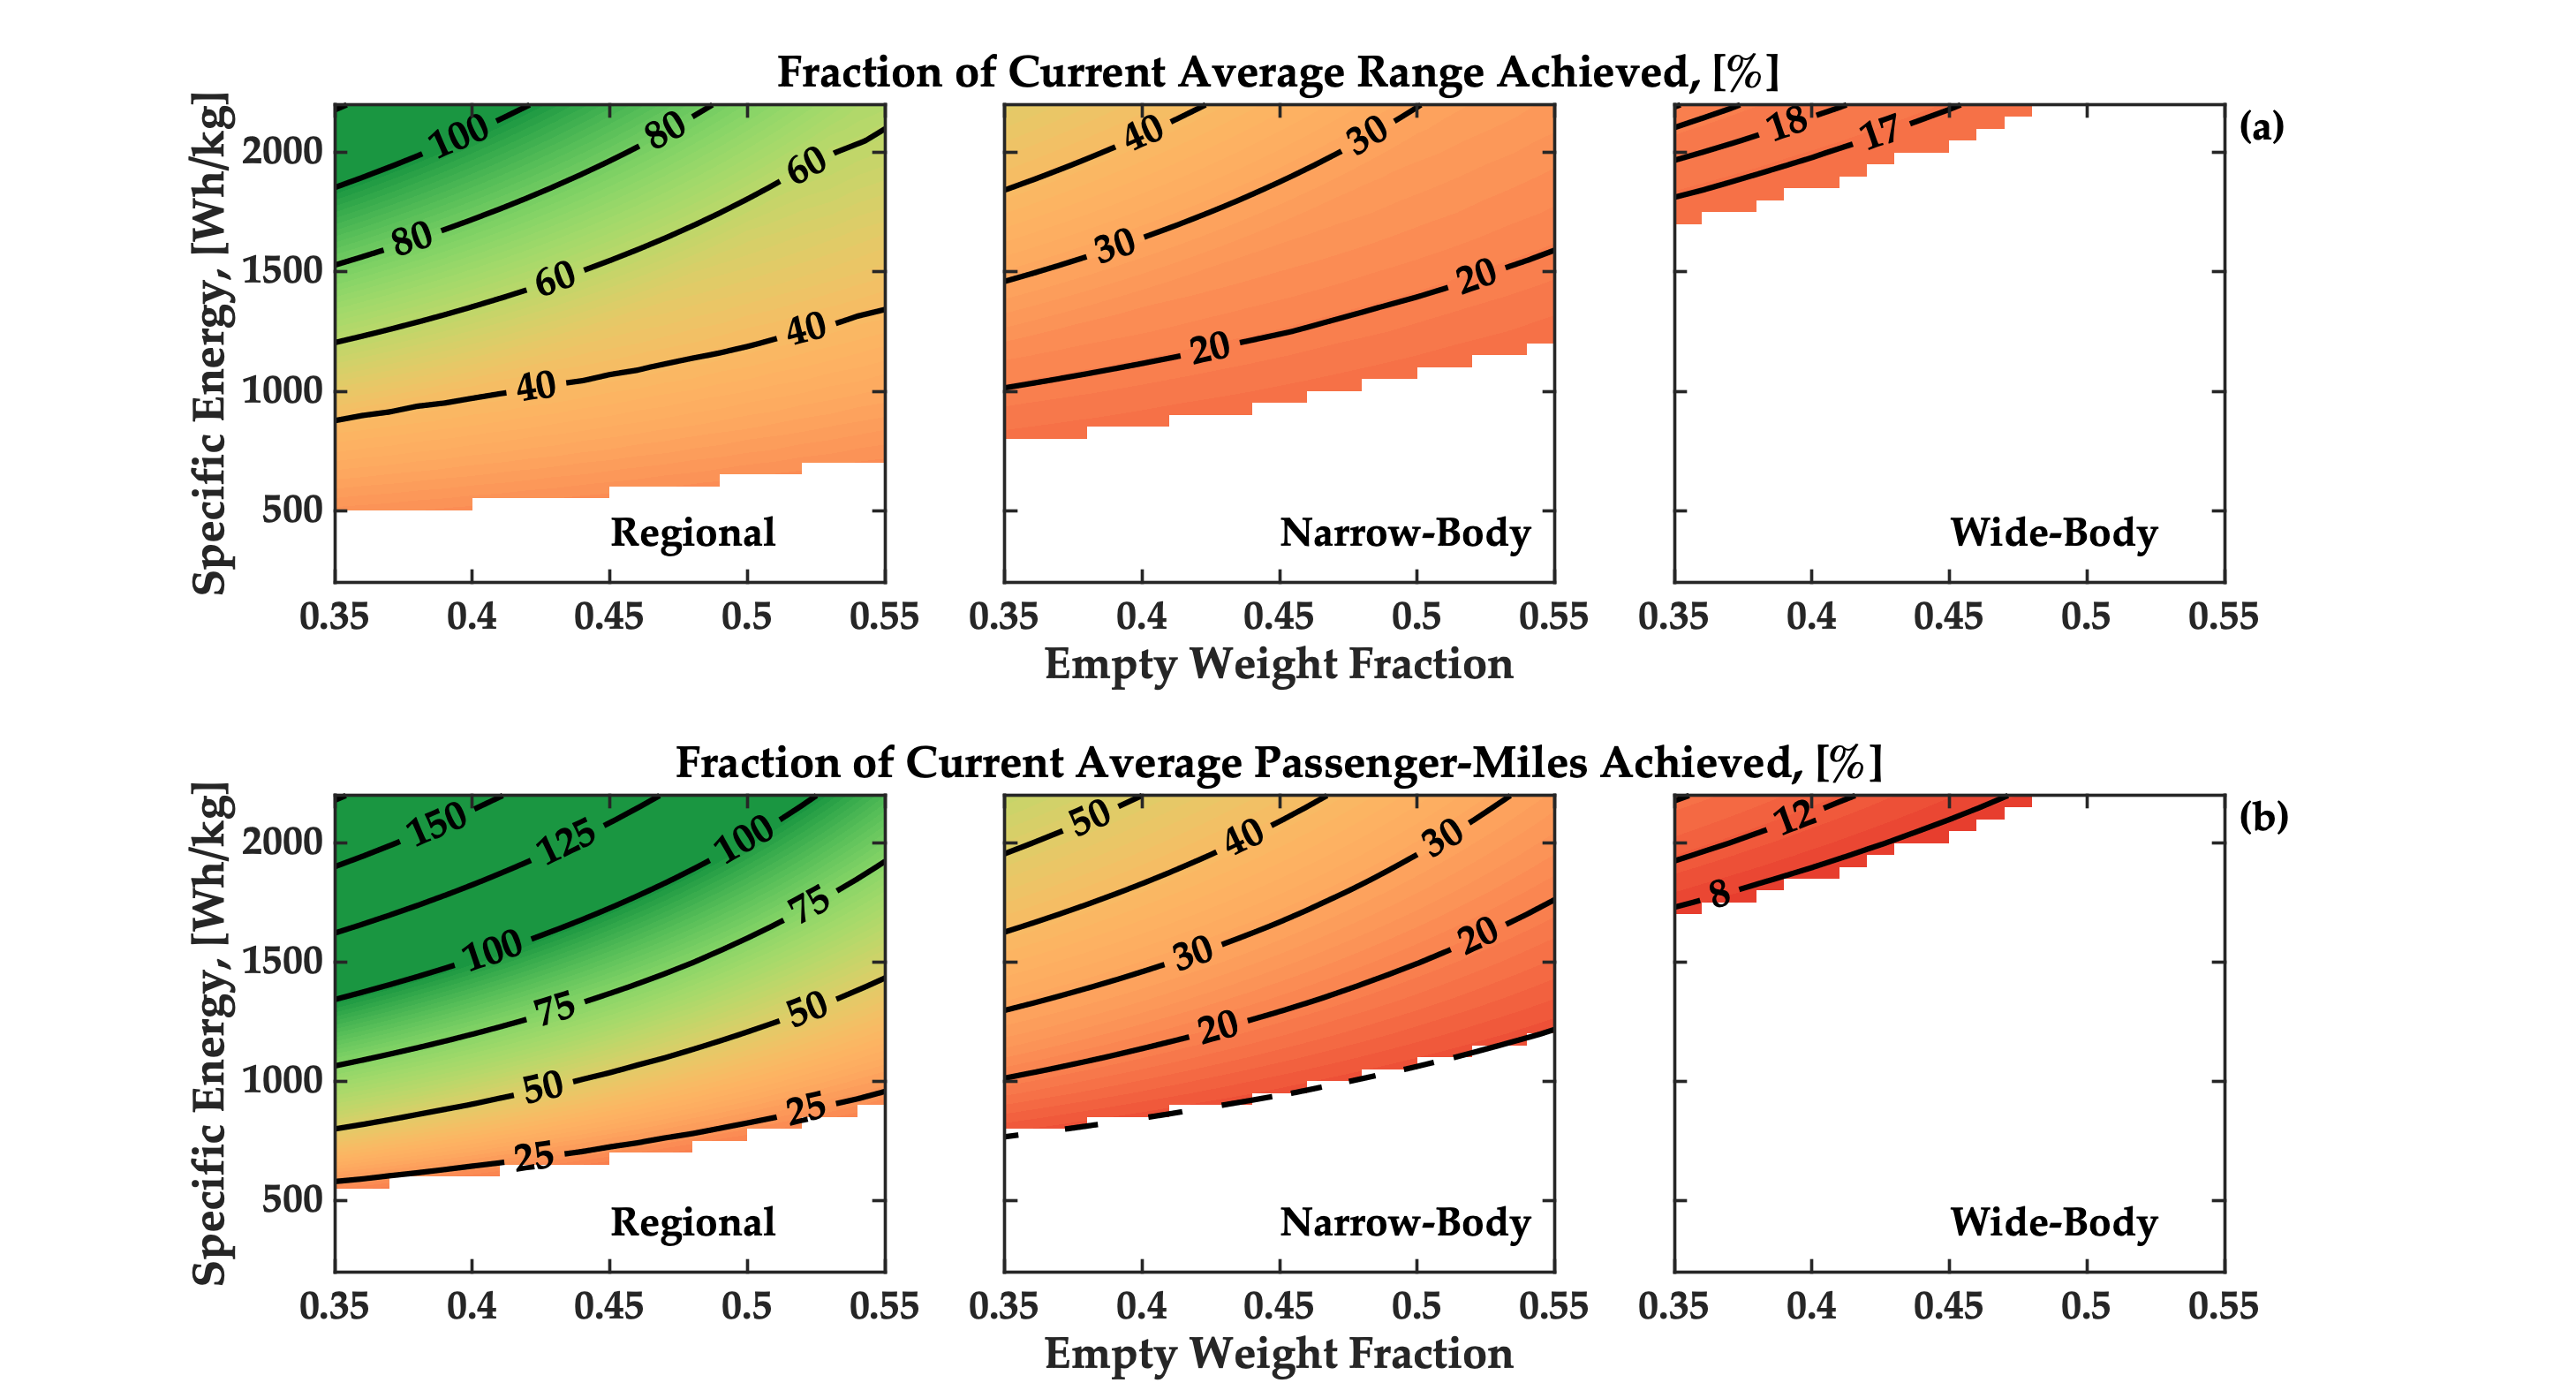
\includegraphics[width=\textwidth]{Figures/contours.png}\hfill
\caption{Range and passenger-miles achieved by electric regional, narrow-body and wide-body aircraft shown as a fraction of the current average range in (a) and passenger-miles in (b) for the respective categories. We observe that for regional aircraft, the current average range is achieved at a pack-level specific energy of about 1,850 Wh/kg and current average passenger-miles at about 1,350 Wh/kg. The threshold for a feasible all-electric regional aircraft is about 500 Wh/kg achieving about 25\% of the current average range. A similar threshold is about 800 Wh/kg and 1,700 Wh/kg for narrow-body and wide-body respectively. However, only 12\% and 16\% of the current average range is achieved at threshold specific energies for the narrow and wide-body aircraft respectively. At the highest pack-level specific energy considered of 2,000 Wh/kg, electric wide-body aircraft can only achieve 19\% and 16\% of current average range and passenger-miles. On the other hand, at 2,000 Wh/kg regional aircraft achieve a much higher range and passenger-miles than the current average.}
\label{fig:contours}
\end{figure}


In all cases considered, the specific energy required of a wide body aircraft is much greater than that of a regional aircraft. This effect is not primarily due to the larger size of the aircraft, but rather to the increased range. To illustrate this effect, consider the power profiles of each of the classes of aircraft for representative ranges flown by each (Figure \ref{fig:powerprofile}). While the size of the aircraft results in the higher power at each point, the energy required to fly the ranges flown by aircraft (the area beneath the curve) increases even more as a result of the increased range. \vv{Good point -- we can make this even more concrete.  Can we now do a hypothetical narrow-body and wide-body at the same range and show what fraction is actually the size effect.  Can we make this visually apparent in Figure 3.}

\begin{figure}[htp]
\centering
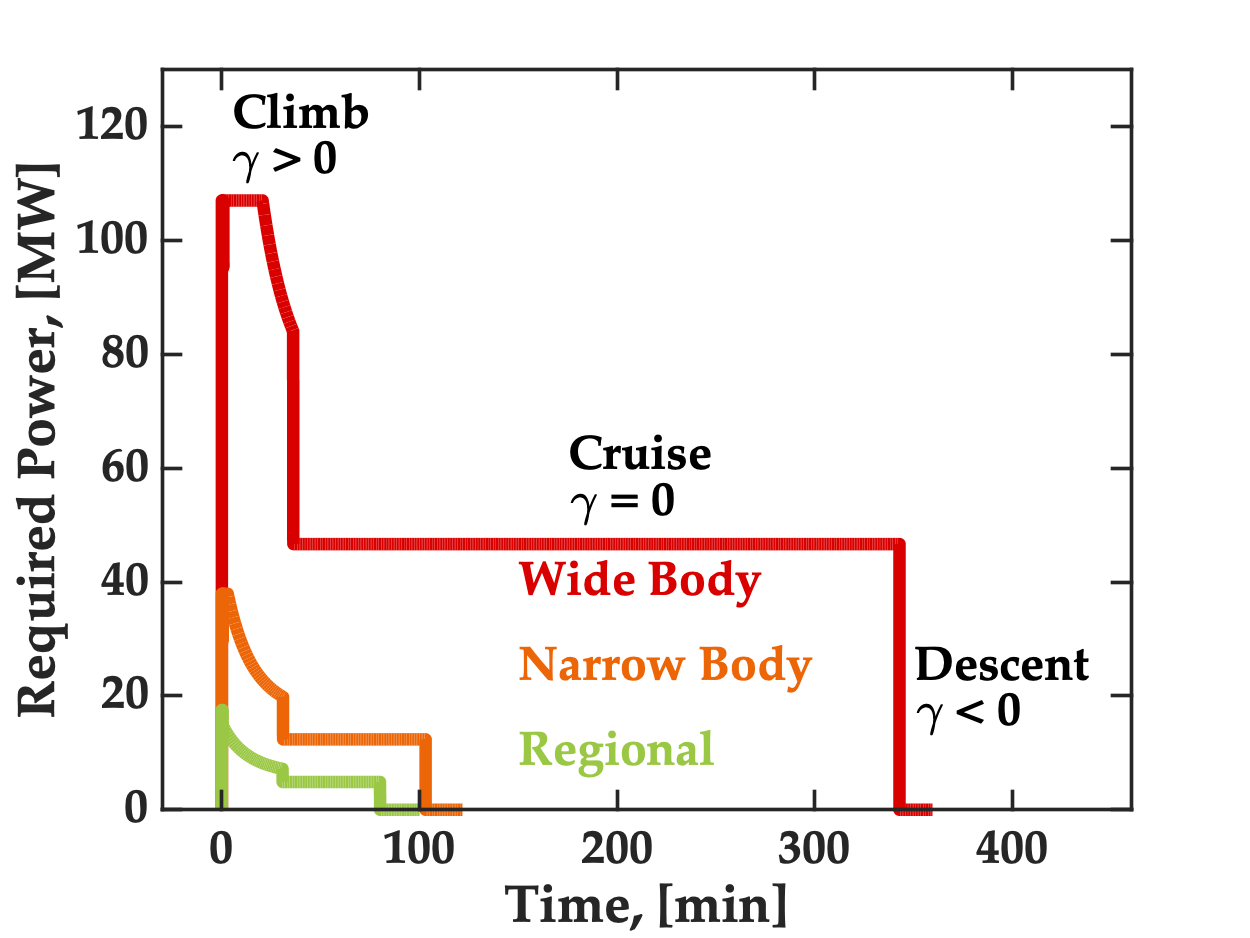
\includegraphics[width=0.6\textwidth]{Figures/powerprofiles.png}
\caption{Aircraft Power Profiles, along with conditions of flight in each segment. This figure illustrates the scaling challenges inherent in electric flight; as MTOM increases, the typical use case range also increases, causing a massive increase in the total energy needed}
\label{fig:powerprofile}
\end{figure}

To find which parameters most affect the performance metrics required for an electric aircraft, a sensitivity analysis was performed. The result is shown in Figure \ref{fig:sensitivity}, where the specific energy is plotted as a function of percentage change from the mean for each parameter to carry out the mission described above.  In each case, the combined efficiency is the most important factor, followed closely by EWF, Drag Coefficient and aspect ratio. Wing loading has a much lower effect on the requirements than do the other parameters. It should be noted here that extensive trade studies are often done in aircraft conceptual design and the effects of these parameters on the power and energy requirements are the primary focus of this paper.

\begin{figure}[htp]

\centering
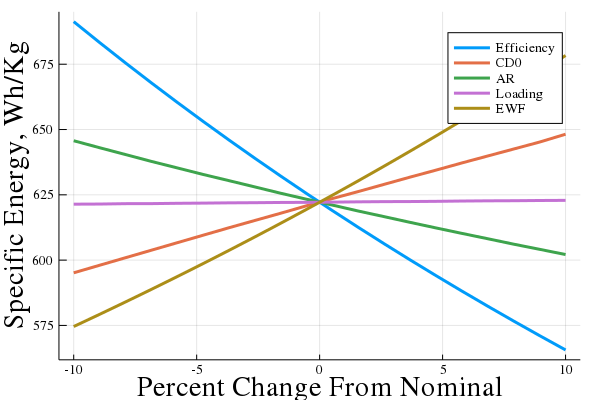
\includegraphics[width=.3\textwidth]{Figures/RJ_Sensitivity.png}\hfill
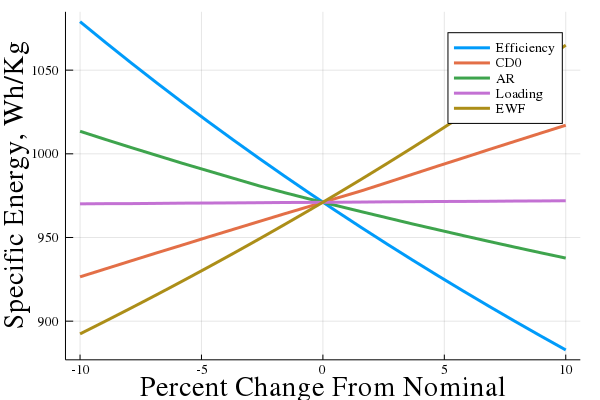
\includegraphics[width=.3\textwidth]{Figures/NB_Sensitivity.png}\hfill
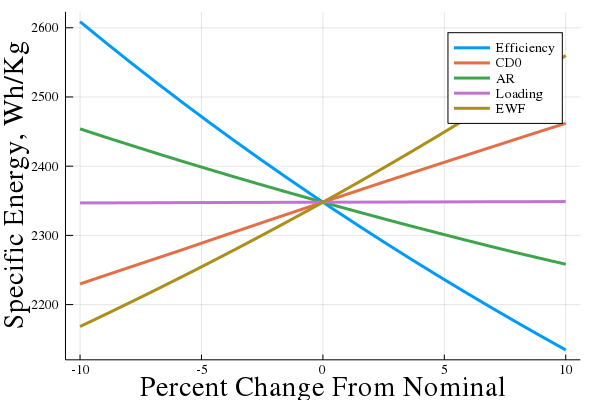
\includegraphics[width=.3\textwidth]{Figures/WB_Sensitivity.png}

\caption{Sensitivity Analysis for regional, narrow body, and wide body aircraft.  \vv{Give more details in the figure caption.  Write a line or two about what's the most important insight from this.}}
\label{fig:sensitivity}

\end{figure}

%\subsection{Discussion of batteries required to meet these requirements, along with discussion of discharge rates}
% \abattention{SHASHANK}
Having identified the energy and power requirements, this allows us now to explore the possible battery chemistries and materials needed to achieve the targets of the three segments of electric aircraft.  For the purpose of this study, we categorize batteries into current `commercial Li-ion batteries', `future Li-ion batteries' including concepts such as silicon or Li-metal based anodes and solid state electrolytes, and `beyond Li-ion batteries' which include chemistries such as Li-S and Li-O$\mathrm{_2}$. The specific energy of current generation Li-ion batteries has steadily increased by about 5\% over the past decade\cite{placke2017lithium} where the current specific energy for commercial Li-ion batteries is about 250 Wh/kg. The projected maximum specific energy values for future Li-ion batteries are around 400 Wh/kg-cell\cite{placke2017lithium} with lithium metal anodes and high voltage and specific capacity cathodes. A cell-level specific energy of 400 Wh/kg is insufficient for the Regional aircraft requirements which are the least stringent among the three categories considered, as seen in the previous discussions. Considering beyond Li-ion batteries, the maximum specific energy of Li-S system is about 500 Wh/kg which reaches the minimum threshold for Regional aircraft. The only other promising chemistry is Li-O$\mathrm{_2}$, where the project maximum specific energies could potentially meet some of the targets estimated previous.

\begin{figure}[h!]
\centering
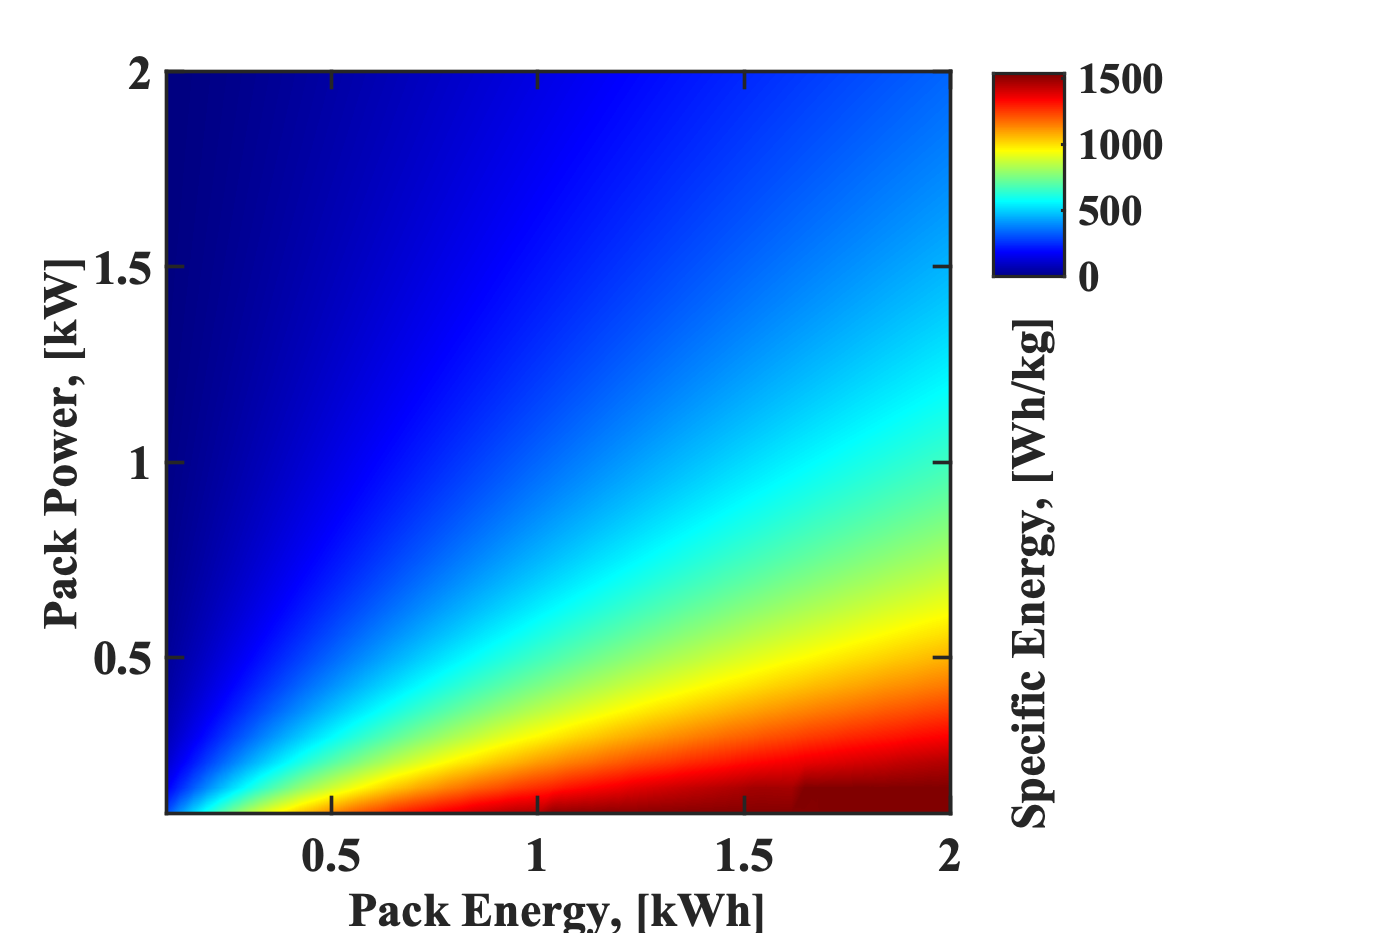
\includegraphics[width=0.7\linewidth]{ragone.png}
\caption{Pack specific energy of Li-air open systems for different pack-level energy and power metrics.}
\label{fig:ragone} 
\end{figure} 

To estimate the cell and pack-level specific energy of Li-O$\mathrm{_2}$ systems, we use previously developed electrochemical and pack design models\cite{gallagher2014quantifying} which were reformulated for the purpose of this study. We examine, an open Li-O$\mathrm{_2}$, which does not carry oxygen on-board to estimate its specific power and energy when the system is designed to meet the demands of the three categories of aircraft. Using the electrochemical and pack design model, we construct a Ragone plot showing the relationship between pack specific energy and specific power, seen in Figure (\ref{fig:ragone})

%\subsection{Future Work, including BLI and Emissions and Money and Stuff}

If these extremely challenging metrics are met, there may be opportunities to lower the emissions associated with commercial aviation. Conventional jet engines emit greenhouse gases such as carbon dioxide, water vapor, nitrous oxides, sulfates and soot when they burn jet fuel. The contrails emitted by aircraft also are a major cause of warming. According to a XXXX paper \textbf{cite whatever madalsa wanted to cite here}, aircraft induced cloudiness causes more than 50\% of the aviation-derived radiative forcing, which directly induces warming in the upper troposphere. While the exact extend of emission savings depends on several factors, including electricity mix, electrifying aircraft would eliminate aircraft induced cloudiness, one of the major contributors to anthropogenic climate change from aviation. 

% Determining the aviation sector’s contribution to anthropogenic climate change is a work-in-progress. One major segment studies greenhouse gas emissions – carbon dioxide, water vapour, nitrous oxides, sulphates, soot - released from burning jet fuel; while others have studied the impact of aircraft-induced cloudiness on the large-scale climate system. There is also a growing body of literature looking at air quality impacts due to fuel burn during aircraft landing and take-off (LTO) for various segments of aviation (NOT ELABORATING AS LTO ENERGY USE IS IGNORED IN OUR TEXT but climate/AQ benefits are plenty) \textbf{(cite lead study, air pollution around airports study, NOx study)}. Electrification of aviation nullifies all three during operation.\\
% While there are challenges to electrify large long-range aircraft at the current state of battery technology \textbf{(cite eipstein)}, smaller aircraft (\textbf{ENTER PAX VALUE OR RANGE DEPENDING ON CONCLUSIONS FROM OUR PAPER)} can reduce carbon emissions by 15\% \textbf{(cite barrett, also added in eipstien}) can serve as starting points for decarbonization of aviation.  \\
% Beyond carbon emissions, it is important to look at the benefits of electrification of aviation by complete removal of Aircraft Induced Cloudiness (AIC) – short term condensation trails (contrails) and long-lived Cirrus homogenitus \textbf{(cite nature paper)}. Within climatic uncertainties, Aircraft induced cloudiness accounts for more than 50\% share in aviation-derived radiative forcing which directly induces warming in upper troposphere. Electrification of aviation would enable rapid and complete mitigation of AICs.

\vv{Conclude with a solid paragraph saying what is needed and what is possible in the near-term, medium-term and long-term.}

%%%%%%%Batteries
%\bibliography{refs}

\vv{Add competing financial interest from eVTOL paper.}
\bibliography{ref.bib}
\end{document}
